\documentclass[12pt]{article}
\usepackage{homework}
\pagestyle{fancy}

% assignment information
\def\course{Statistical Mechanics}
\def\assignmentno{Problem Sheet 2}
\def\assignmentname{Magnets and Oscillators}
\def\name{Xin, Wenkang}
\def\time{\today}

\begin{document}

\begin{titlepage}
    \begin{center}
        \large
        \textbf{\course}

        \vfill

        \Huge
        \textbf{\assignmentno}

        \vspace{1.5cm}

        \large{\assignmentname}

        \vfill

        \large
        \name

        \time
    \end{center}
\end{titlepage}


%==========
\pagebreak
\section*{Magnets and oscillators}
%==========


\problem{2.1}{}

\subproblem{i}
The energy levels are given by:

\begin{equation}
    E_{\pm} = \pm \mu_{B} B
\end{equation}

The single particle partition function is:

\begin{equation}
    Z_{1} = e^{-\beta \mu_{B} B} + e^{\beta \mu_{B} B} = 2 \cosh{(\beta \mu_{B} B)}
\end{equation}

\subproblem{ii}{}
The partition function for $N$ non-interacting particles is:

\begin{equation}
    Z = Z_{1}^{N} = [2 \cosh{(\beta \mu_{B} B)}]^{N}
\end{equation}

so that the internal energy is:

\begin{equation}
    \begin{split}
        U &= -\frac{\partial \ln{Z}}{\partial \beta} \\
        &= -N \frac{\partial \ln{[2 \cosh{(\beta \mu_{B} B)}]}}{\partial \beta} \\
        &= -N \mu_{B} B \tanh{(\beta \mu_{B} B)}
    \end{split}
\end{equation}

The heat capacity is:

\begin{equation}
    C_{B} = \left( \frac{\partial U}{\partial T} \right)_{B} = N k_{B} \left( \frac{\theta}{T} \right)^{2} \frac{1}{\cosh^{2}{(\theta/T)}}
\end{equation}

where we identify the temperature scale:

\begin{equation}
    \theta \equiv \frac{\mu_{B} B}{k_{B}}
\end{equation}

The maximum of $C_{B}$ can be derived by setting the derivative to zero. Denoting $x = \theta/T$, we have:

\begin{equation}
    \begin{split}
        \frac{\partial C_{B}}{\partial x} &\propto -2x^{2} \frac{\sinh{x}}{\cosh^{3}{x}} + 2x \frac{1}{\cosh^{2}{x}} \\
        &= 2x \frac{1 - x \tanh{x}}{\cosh^{2}{x}} \\
    \end{split}
\end{equation}

Thus, the maximum of $C_{B}$ occurs at $x = \tanh{x}$, which is approximately $x = 1.20$. Therefore, the maximum of $C_{B}$ occurs at:

\begin{equation}
    T_{\text{peak}} = \frac{\theta}{1.20} = 0.83 \frac{\mu_{B} B}{k_{B}}
\end{equation}

\subproblem{iii}{}
With $B = \qty{2}{T}$ and $\mu_{B} = \qty{9.27e-24}{J/T}$, we have:

\begin{equation}
    T_{\text{peak}} = \qty{1.119}{K}
\end{equation}

at which the heat capacity of the system is significant.

\subproblem{iv}{}
At high $T$, we have $\theta/T \ll 1$, so that $\cosh{(\theta/T)} \approx 1$ and $C_{B} \propto T^{-2}$. At low $T$, we have $\theta/T \gg 1$, so that:

\begin{equation}
    C_{B} \propto \frac{1}{T^{2}} \frac{e^{\theta/T}}{e^{2\theta/T}} \propto \frac{e^{-\theta/T}}{T^{2}}
\end{equation}
\qed


\problem{2.2}{}
The partition function for a single particle in a harmonic oscillator potential is:

\begin{equation}
    Z_{1} = \sum_{n=0}^{\infty} e^{-\beta \hbar \omega (n + 1/2)} = \frac{e^{-\beta \hbar \omega/2}}{1 - e^{-\beta \hbar \omega}} = \frac{1}{2 \sinh{\left( \beta \hbar \omega / 2 \right)}}
\end{equation}

The partition function for $N$ non-interacting particles is:

\begin{equation}
    Z = Z_{1}^{N} = \frac{1}{\left[ 2 \sinh{\left( \beta \hbar \omega / 2 \right)} \right]^{N}}
\end{equation}

The internal energy is:

\begin{equation}
    \begin{split}
        U &= -\left( \frac{\partial \ln Z}{\partial \beta} \right)_{V} \\
        &= \frac{N \hbar \omega}{2} + \frac{N \hbar \omega}{\exp\left( \beta \hbar \omega \right) - 1}
    \end{split}
\end{equation}

so that the specific heat is:

\begin{equation}
    C_{V} = \left( \frac{\partial U}{\partial T} \right)_{V} = N k_{B} \left( \frac{\hbar \omega}{k_{B}T} \right)^{2} \frac{\exp\left( \beta \hbar \omega \right)}{\left[ \exp\left( \beta \hbar \omega \right) - 1 \right]^{2}} = N k_{B} \left[ \frac{\beta \hbar \omega/2}{\sinh\left( \beta \hbar \omega / 2 \right)} \right]^{2}
\end{equation}

In high temperature limit, we have $\beta \hbar \omega \ll 1$, so that $C_{V} \to N k_{B}$. In low temperature limit, we have $\beta \hbar \omega \gg 1$, so that $C_{V} \to 0$.
\qed


\problem{2.3}{}
The free energy of a single particle in a harmonic oscillator potential is:

\begin{equation}
    F_{1} = -k_{B}T \ln{Z_{1}} = -k_{B}T \ln{\left[ \frac{1}{2 \sinh{\left( \beta \hbar \omega / 2 \right)}} \right]}
\end{equation}

so that the entropy (scaled by $k_{B}$) is:

\begin{equation}
    \frac{S_{1}}{k_{B}} = -\frac{1}{k_{B}} \left( \frac{\partial F_{1}}{\partial T} \right)_{V} = \ln{\left[ \frac{1}{2 \sinh{\left( \theta / T \right)}} \right]} + \frac{\theta}{T} \frac{\cosh{\left( \theta / T \right)}}{\sinh{\left( \theta / T \right)}}
\end{equation}

where we define the temperature scale $\theta \equiv \hbar \omega / 2k_{B}$.

We require the internal energy of system, defined as:

\begin{equation}
    U = -\left( \frac{\partial \ln{Z_{1}}}{\partial \beta} \right)_{V} = \frac{\hbar \omega}{2} + \frac{\hbar \omega}{\exp\left( 2\theta / T \right) - 1}
\end{equation}

to equal $(m + 1/2)\hbar \omega$.

This puts a constraint on the temperature:

\begin{equation}
    \frac{1}{\exp\left( 2\theta / T \right) - 1} = m
\end{equation}

or equivalently $e^{2\theta / T} = 1 + 1/m$.

Substituting this into the entropy expression, we have:

\begin{equation}
    \begin{split}
        \frac{S_{1}}{k_{B}} &= -\ln{\left( \sqrt{1 + 1/m} - \frac{1}{\sqrt{1 + 1/m}} \right)} + (1 + 2m) \ln{\sqrt{1 + 1/m}} \\
        &= -\ln{\left( \frac{1}{\sqrt{m^{2} + m}} \right)} + (1 + 2m) \ln{\sqrt{1 + 1/m}} \\
        &= (m + 1) \ln{(m + 1)} - m \ln{m}
    \end{split}
\end{equation}

which is the desired result.

When $m \to 0$, we have $S_{1} \to 0$. This means that the entropy is zero (which is an arbitrary reference value) when every particle is in the ground state.
\qed


\problem{2.4}{}

\subproblem{i}
The single particle partition function is:

\begin{equation}
    \begin{split}
        Z_{M} &= \sum_{k = -J}^{J} \exp \left( \beta k g_{J} \mu_{B} B \right) \\
        &= \sum_{k = -J}^{J} \exp \left( k C \right) \\
        &= \frac{e^{-J C} - e^{(J+1)C}}{1 - e^{C}} \\
        &= \frac{\sinh{\left[ ( J + 1/2 ) C \right]}}{\sinh{\left( C/2 \right)}}
    \end{split}
\end{equation}

where $C \equiv g_{J} \mu_{B} B / k_{B} T$.

\subproblem{ii}{}
Consider the free energy for $\mathcal{N} = NV$ particles:

\begin{equation}
    F = \mathcal{N} F_{1} = -\mathcal{N} k_{B} T \ln{Z_{M}}
\end{equation}

The total magnetic moment is:

\begin{equation}
    m = -\mathcal{N} \left( \frac{\partial F_{1}}{\partial B} \right)_{T}
\end{equation}

so that the magnetization is:

\begin{equation}
    \begin{split}
        M &= \frac{m}{V} \\
        &= -N \left( \frac{\partial F_{1}}{\partial B} \right)_{T} \\
        &= -N \frac{g_{J} \mu_{B}}{k_{B} T} \left( \frac{\partial F_{1}}{\partial C} \right)_{T} \\
        &= N g_{J} \mu_{B} \left[ \frac{J + 1/2}{\tanh{[(J + 1/2)C]}} - \frac{1/2}{\tanh{(C/2)}} \right] \\
        &= N g_{J} \mu_{B} \frac{1}{C} \left[ \frac{(J + 1/2)C}{\tanh{[(J + 1/2)C]}} - \frac{C/2}{\tanh{(C/2)}} \right]
    \end{split}
\end{equation}

Thus, the susceptibility can be taken as:

\begin{equation}
    \begin{split}
        \chi &= \frac{\mu_{0} M}{B} \\
        &= \frac{\mu_{0} N g_{J}^{2} \mu_{B}^{2}}{k_{B}T} \frac{1}{C^{2}} \left[ \frac{(J + 1/2)C}{\tanh{[(J + 1/2)C]}} - \frac{C/2}{\tanh{(C/2)}} \right] \\
        &\approx \frac{\mu_{0} N g_{J}^{2} \mu_{B}^{2}}{k_{B}T} \frac{1}{C^{2}} \left( \frac{[(J + 1/2)C]^{2}}{3} - \frac{C^{2}/4}{3} \right) \\
        &= \frac{\mu_{0} N g_{J}^{2} \mu_{B}^{2}}{3 k_{B}T} J(J + 1)
    \end{split}
\end{equation}

which reduces to the Curie law for $J = 1/2$.

\subproblem{iii}{}
Define the partition function for a harmonic oscillator as:

\begin{equation}
    Z_{\text{SHO}}(\hbar \omega) = \frac{1}{2 \sinh{(\beta \hbar \omega / 2)}}
\end{equation}

We can check that $Z_{M}$ is a ratio of two partition functions:

\begin{equation}
    Z_{M} = \frac{Z_{\text{SHO}}(g_{J} \mu_{B} B)}{Z_{\text{SHO}}[(2J + 1)g_{J} \mu_{B} B]}
\end{equation}

Consider the logarithm of $-Z_{M}$:

\begin{equation}
    -\ln{Z_{M}} = -\ln{Z_{\text{SHO}}(g_{J} \mu_{B} B)} + \ln{Z_{\text{SHO}}[(2J + 1)g_{J} \mu_{B} B]}
\end{equation}

This means that the free energy is that of a harmonic oscillator with frequency $g_{J} \mu_{B} B$ minus that of a harmonic oscillator with frequency $(2J + 1)g_{J} \mu_{B} B$.

\subproblem{iv}{}
Given the form of $Z_{M}$ as a ratio of harmonic oscillator partition functions, we can write the internal energy as:

\begin{equation}
    \begin{split}
        U &= -\left( \frac{\partial \ln{Z_{M}}}{\partial \beta} \right)_{V} \\
        &= -\left( \frac{\partial \ln{Z_{\text{SHO}}(g_{J} \mu_{B} B)}}{\partial \beta} \right)_{V} + \left( \frac{\partial \ln{Z_{\text{SHO}}[(2J + 1)g_{J} \mu_{B} B]}}{\partial \beta} \right)_{V} \\
        &= U_{\text{SHO}}(g_{J} \mu_{B} B) - U_{\text{SHO}}[(2J + 1)g_{J} \mu_{B} B]
    \end{split}
\end{equation}

This implies that the heat capacity can be written as a difference of those for the two harmonic oscillators:

\begin{equation}
    \begin{split}
        C_{V} &= \left( \frac{\partial U}{\partial T} \right)_{V} \\
        &= C_{V, \text{SHO}}(g_{J} \mu_{B} B) - C_{V, \text{SHO}}[(2J + 1)g_{J} \mu_{B} B] \\
        &= k_{B} \left[ \frac{\beta \hbar \omega_{1}/2}{\sinh\left( \beta \hbar \omega_{1}/2 \right)} \right]^{2} - k_{B} \left[ \frac{\beta \hbar \omega_{2}/2}{\sinh\left( \beta \hbar \omega_{2}/2 \right)} \right]^{2}
    \end{split}
\end{equation}

where for simplicity we define the frequencies:

\begin{equation}
    \hbar \omega_{1} \equiv g_{J} \mu_{B} B \qquad \hbar \omega_{2} \equiv (2J + 1)g_{J} \mu_{B} B
\end{equation}

We can define the temperature scale:

\begin{equation}
    \phi \equiv \frac{\hbar \omega}{k_{B}} = \frac{g_{J} \mu_{B} B}{k_{B}}
\end{equation}

so that the heat capacity becomes:

\begin{equation}
    C_{V} = k_{B} \left[ \frac{\phi/2}{\sinh\left( \phi/2 \right)} \right]^{2} - k_{B} \left[ \frac{(2J + 1)\phi/2}{\sinh\left[ (2J + 1)\phi/2 \right]} \right]^{2}
\end{equation}

\begin{figure}[!h]
    \centering
    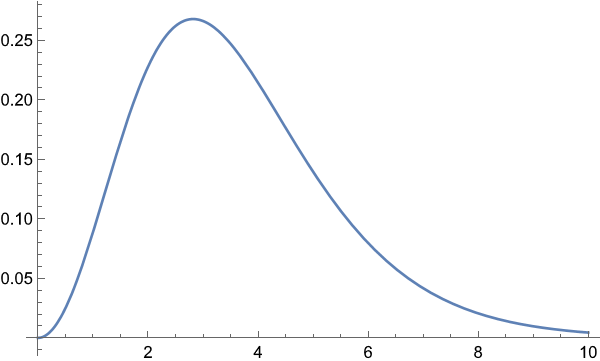
\includegraphics[width=0.32\textwidth]{../plots/statistics_2_4_a.png}
    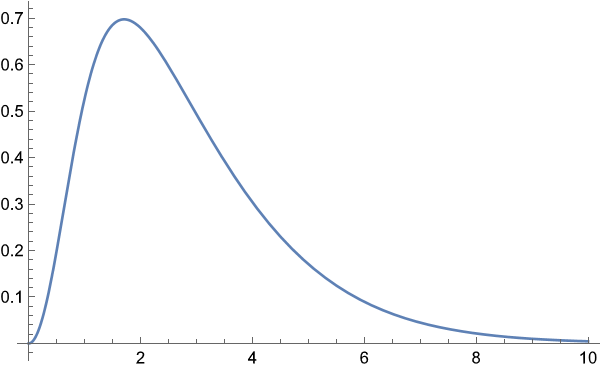
\includegraphics[width=0.32\textwidth]{../plots/statistics_2_4_b.png}
    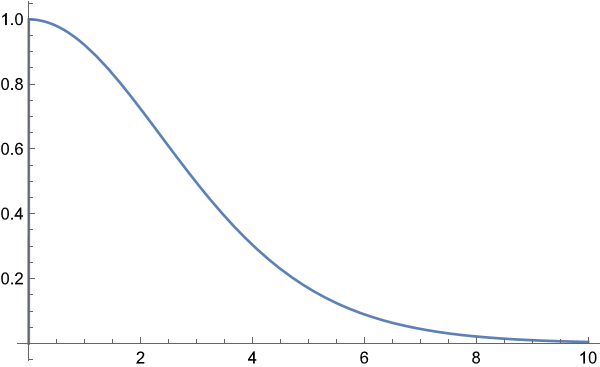
\includegraphics[width=0.32\textwidth]{../plots/statistics_2_4_c.png}
    \caption{Heat capacity for $J = 1/2$, $J = 3/2$ and $J \to \infty$.}
\end{figure}

As shown in the figures, higher $J$ shifts the maximum of the heat capacity towards lower temperatures. In the limit $J \to \infty$, the heat capacity peaks at $T = 0$. Therefore, it is possible to plot the heat capacity as a function of $T$ for a given system and determine $J$ from the position of the peak.
\qed


\problem{2.5}{}

\subproblem{i}
Consider a single three-dimensional harmonic oscillator with characteristic frequencies $\omega_{i}$, $i = 1, 2, 3$. The energy levels are given by:

\begin{equation}
    E_{n_{1}, n_{2}, n_{3}} = \hbar \omega_{1} \left( n_{1} + \frac{1}{2} \right) + \hbar \omega_{2} \left( n_{2} + \frac{1}{2} \right) + \hbar \omega_{3} \left( n_{3} + \frac{1}{2} \right)
\end{equation}

The single particle partition function, denoted $Z_{1}^{(3)}$, is:

\begin{equation}
    \begin{split}
        Z_{1}^{(3)} &= \sum_{n_{1}, n_{2}, n_{3}} e^{-\beta E_{n_{1}, n_{2}, n_{3}}} \\
        &= \sum_{n_{1}} e^{-\beta \hbar \omega_{1} \left( n_{1} + \frac{1}{2} \right)} \sum_{n_{2}} e^{-\beta \hbar \omega_{2} \left( n_{2} + \frac{1}{2} \right)} \sum_{n_{3}} e^{-\beta \hbar \omega_{3} \left( n_{3} + \frac{1}{2} \right)} \\
        &= Z_{1, x} Z_{1, y} Z_{1, z}
    \end{split}
\end{equation}

Assuming identical frequencies $\omega_{i} = \omega$, we have:

\begin{equation}
    Z_{1}^{(3)} = Z_{1}^{3}
\end{equation}

Then the partition function for $N$ non-interacting three-dimensional harmonic oscillators is:

\begin{equation}
    Z^{(3)} = (Z_{1}^{(3)})^{N} = (Z_{1}^{3})^{N} = Z_{1}^{3N}
\end{equation}

Since the partition function contains all information about the thermodynamics of the system, $N$ non-interacting three-dimensional harmonic oscillators is equivalent to $3N$ one-dimensional harmonic oscillators.

\subproblem{ii}{}
Given $\omega = 2\pi \nu = \qty{3.3e13}{rad s^{-1}}$, we have the specific heat:

\begin{equation}
    C_{V} = 3N k_{B} \left[ \frac{\beta \hbar \omega/2}{\sinh\left( \beta \hbar \omega / 2 \right)} \right]^{2}
\end{equation}

Defining the temperature scale $\theta \equiv \hbar \omega / 2k_{B} = \qty{124.8}{K}$, we have:

\begin{equation}
    C_{V} = 3N k_{B} \left[ \frac{\theta/T}{\sinh\left( \theta/T \right)} \right]^{2}
\end{equation}

The function $x^{2}/\sinh^{2}{x}$ has a maximum of unity at $x = 0$, so the maximum of $C_{V}$ is $3Nk_{B}$ as $T \to \infty$. At room temperature (taken as $T_{\text{room}} = \qty{298}{K}$), we have:

\begin{equation}
    \frac{C_{V}}{3Nk_{B}} = \left[ \frac{\theta/T_{\text{room}}}{\sinh\left( \theta/T_{\text{room}} \right)} \right]^{2} \approx 0.94
\end{equation}

This means that the specific heat of the system is already significant at room temperature.

\subproblem{iii}{}
We make the change to temperature scale:

\begin{equation}
    \theta = \frac{\hbar \omega}{2k_{B}} = \qty{748.7}{K}
\end{equation}

The new fraction for the heat capacity is:

\begin{equation}
    \frac{C_{V}}{3Nk_{B}} = \left[ \frac{\theta/T_{\text{room}}}{\sinh\left( \theta/T_{\text{room}} \right)} \right]^{2} \approx 0.017
\end{equation}

which is significantly smaller due to a higher temperature scale.
\qed


\problem{2.6}{}

\subproblem{i}
Suppose that out of the total $N$ particles, $rN$ are the in the higher energy state $E_{+}$ and $(1-r)N$ are in the lower energy state $E_{-}$. We assume $r > 0.5$. We could write the entropy as:

\begin{equation}
    S = -k_{B} \sum_{-, +} p_{i} \ln{p_{i}} = -k_{B} \left[ r \ln{r} + (1-r) \ln{(1-r)} \right]
\end{equation}

and the internal energy:

\begin{equation}
    U = rN E_{+} + (1-r)N E_{-}
\end{equation}

But the temperature is defined via the entropy as:

\begin{equation}
    \begin{split}
        T &= -\left( \frac{\partial U}{\partial S} \right)_{V} \\
        &= -\left( \frac{\partial U}{\partial r} \right)_{V} \left( \frac{\partial r}{\partial S} \right)_{V} \\
        &= \frac{N(E_{+} - E_{-})}{k_{B} [\ln{r} - \ln{(1-r)}]}
    \end{split}
\end{equation}

Since $r > 1 - r$ and both quantities are less than unity, we have $\ln{r} - \ln{(1-r)} < 0$. Therefore, the effective temperature is negative, which shows that the system \mistake{cannot be in equilibrium}.

\begin{correction}
    Note the second derivative of the entropy with respect to $U$:

    \begin{equation}
        \begin{split}
            \left( \frac{\partial^{2} S}{\partial U^{2}} \right)_{V} &= -\left[ \frac{\partial (1/T)}{\partial U} \right]_{V} \\
            &= -\left[ \frac{\partial (1/T)}{\partial r} \right]_{V} \left( \frac{\partial r}{\partial U} \right)_{V} \\
            &= -\frac{k_{B}}{N^{2}(E_{+} - E_{-})^{2}} \left( \frac{1}{r} + \frac{1}{1 - r} \right)
        \end{split}
    \end{equation}

    Since this is a negative quantity, the system is still in equilibrium, i.e., $C_{V} > 0$.
\end{correction}

\subproblem{ii}{}
The swapping operation is equivalent to the exchange of the ratios $r$ and $1-r$, i.e., the substitution $r \to 1-r$. The entropy is invariant under this operation, but the temperature changes sign:

\begin{equation}
    T \to \frac{E_{+} - E_{-}}{k_{B} [\ln{(1-r)} - \ln{r}]}
\end{equation}

\subproblem{iii}{}
Taking instead the limit $r \to 1$, we have $\ln{r} \to 0$ and $\ln{(1-r)} \to -\infty$, so that the temperature tends to zero:

\begin{equation}
    T \to -\frac{E_{+} - E_{-}}{k_{B} \ln{(1-r)}} \to 0
\end{equation}
\qed


\end{document}